% Appendix C

\chapter{Time Management} % Main appendix title

\label{AppendixC} % For referencing this appendix elsewhere, use \ref{AppendixA}

\lhead{Appendix C. \emph{Time Management}} % This is for the header on each page - perhaps a shortened title

\lstdefinestyle{DOS}
{
    backgroundcolor=\color{black},
    basicstyle=\scriptsize\color{white}\ttfamily
    numbers=none,
    numbersep=8pt,                   % how far the line-numbers are from the code
    numberstyle=\tiny\color{white}, % the style that is used for the line-numbers
    stepnumber=1                    % the step between two line-numbers. If it's 1, each line will be numbered
}
%----------------------------------------------------------------------------------------
\lstdefinestyle{C}
{
  morekeywords={export}
}
%----------------------------------------------------------------------------------------

This appendix presents a task list through the practice period and its corresponding Gantt diagram.

Generally speaking, most tasks were finished as they had had been scheduled. Especially in the first two months, time spent on bibliography work was much less than it had been estimated. 

Major delay came from the implementation of object-oriented programming on GPUs and dynamic allocations. This part of work should have been done within one month. Unfortunately, it hasn't been finished during the internship. To a certain extent, other reasons like no available working computer in the first week or contacting researchers in the USA for technical supports postponed the advancement as well. Furthermore, the report redaction lasted for about one month.
\begin{figure}[htbp]
	\centering
		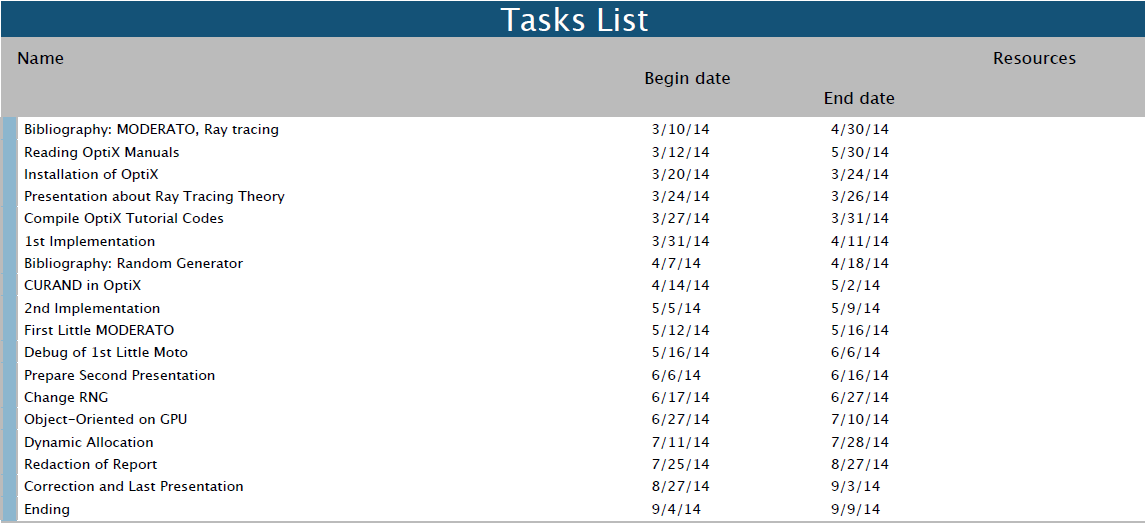
\includegraphics[width=10cm]{Figures/task.png}
	\caption{Task list.}
\end{figure}
\begin{figure}[htbp]
	\centering
		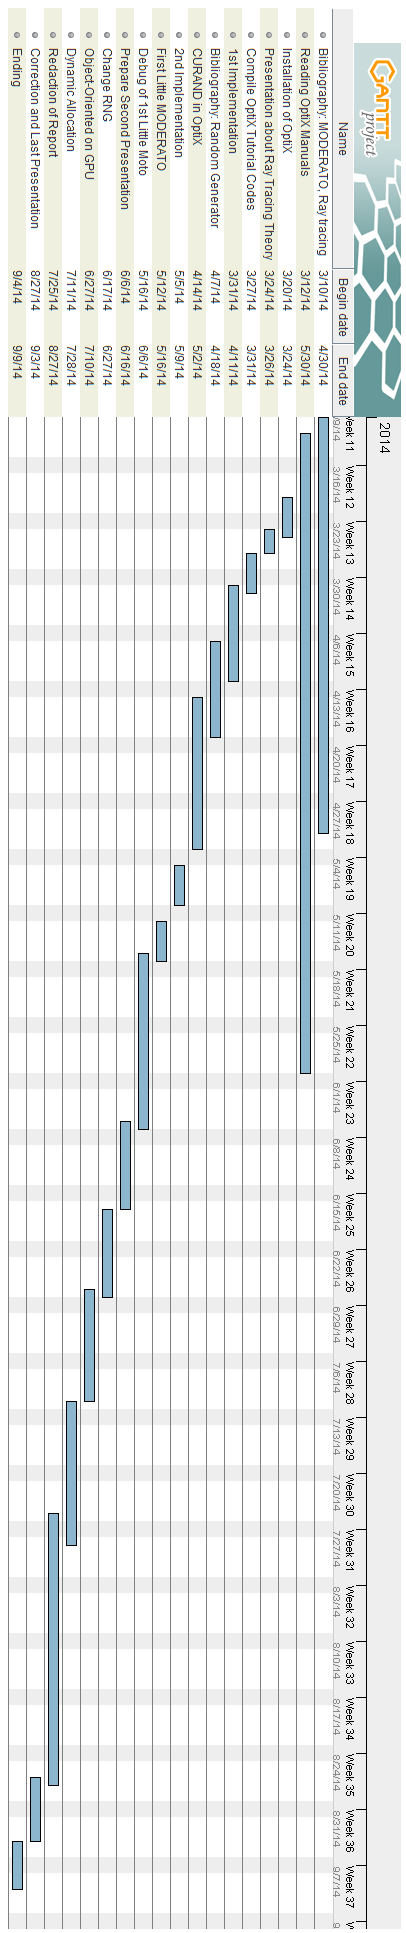
\includegraphics[width=\textwidth,height=\textheight,keepaspectratio]{Figures/report.png}
	\caption{Gantt diagram.}
\end{figure}